%!TEX root =  main.tex
\section{Appendix: Validity under unequal $n_j$}\label{app:unequal}

Consider a specific setting in which $N = 800$, $\sigma = 0.1$, and $k = 4$. Figure~\ref{Fig:unequal-group-sizes} shows the reference distributions of $F_1$ in four scenarios, each with a different group allocation of the 800 observations. The distribution in $s_0$, the equal group size scenario, generally takes the highest values; indeed it exceeds the other scenarios at every quantile. This represents the distribution that we use to calculate $p$-values and reject $H_0$ whenever an observed statistic is greater than the vertical dotted line (when $\alpha = .05$). This means that in the other three scenarios, featuring unequal allocation, the actual type I error rate (the proportion of the distributions beyond the dotted line) will be less than $\alpha$ and we meet the condition for valid $p$-values.

\begin{figure}
\centering
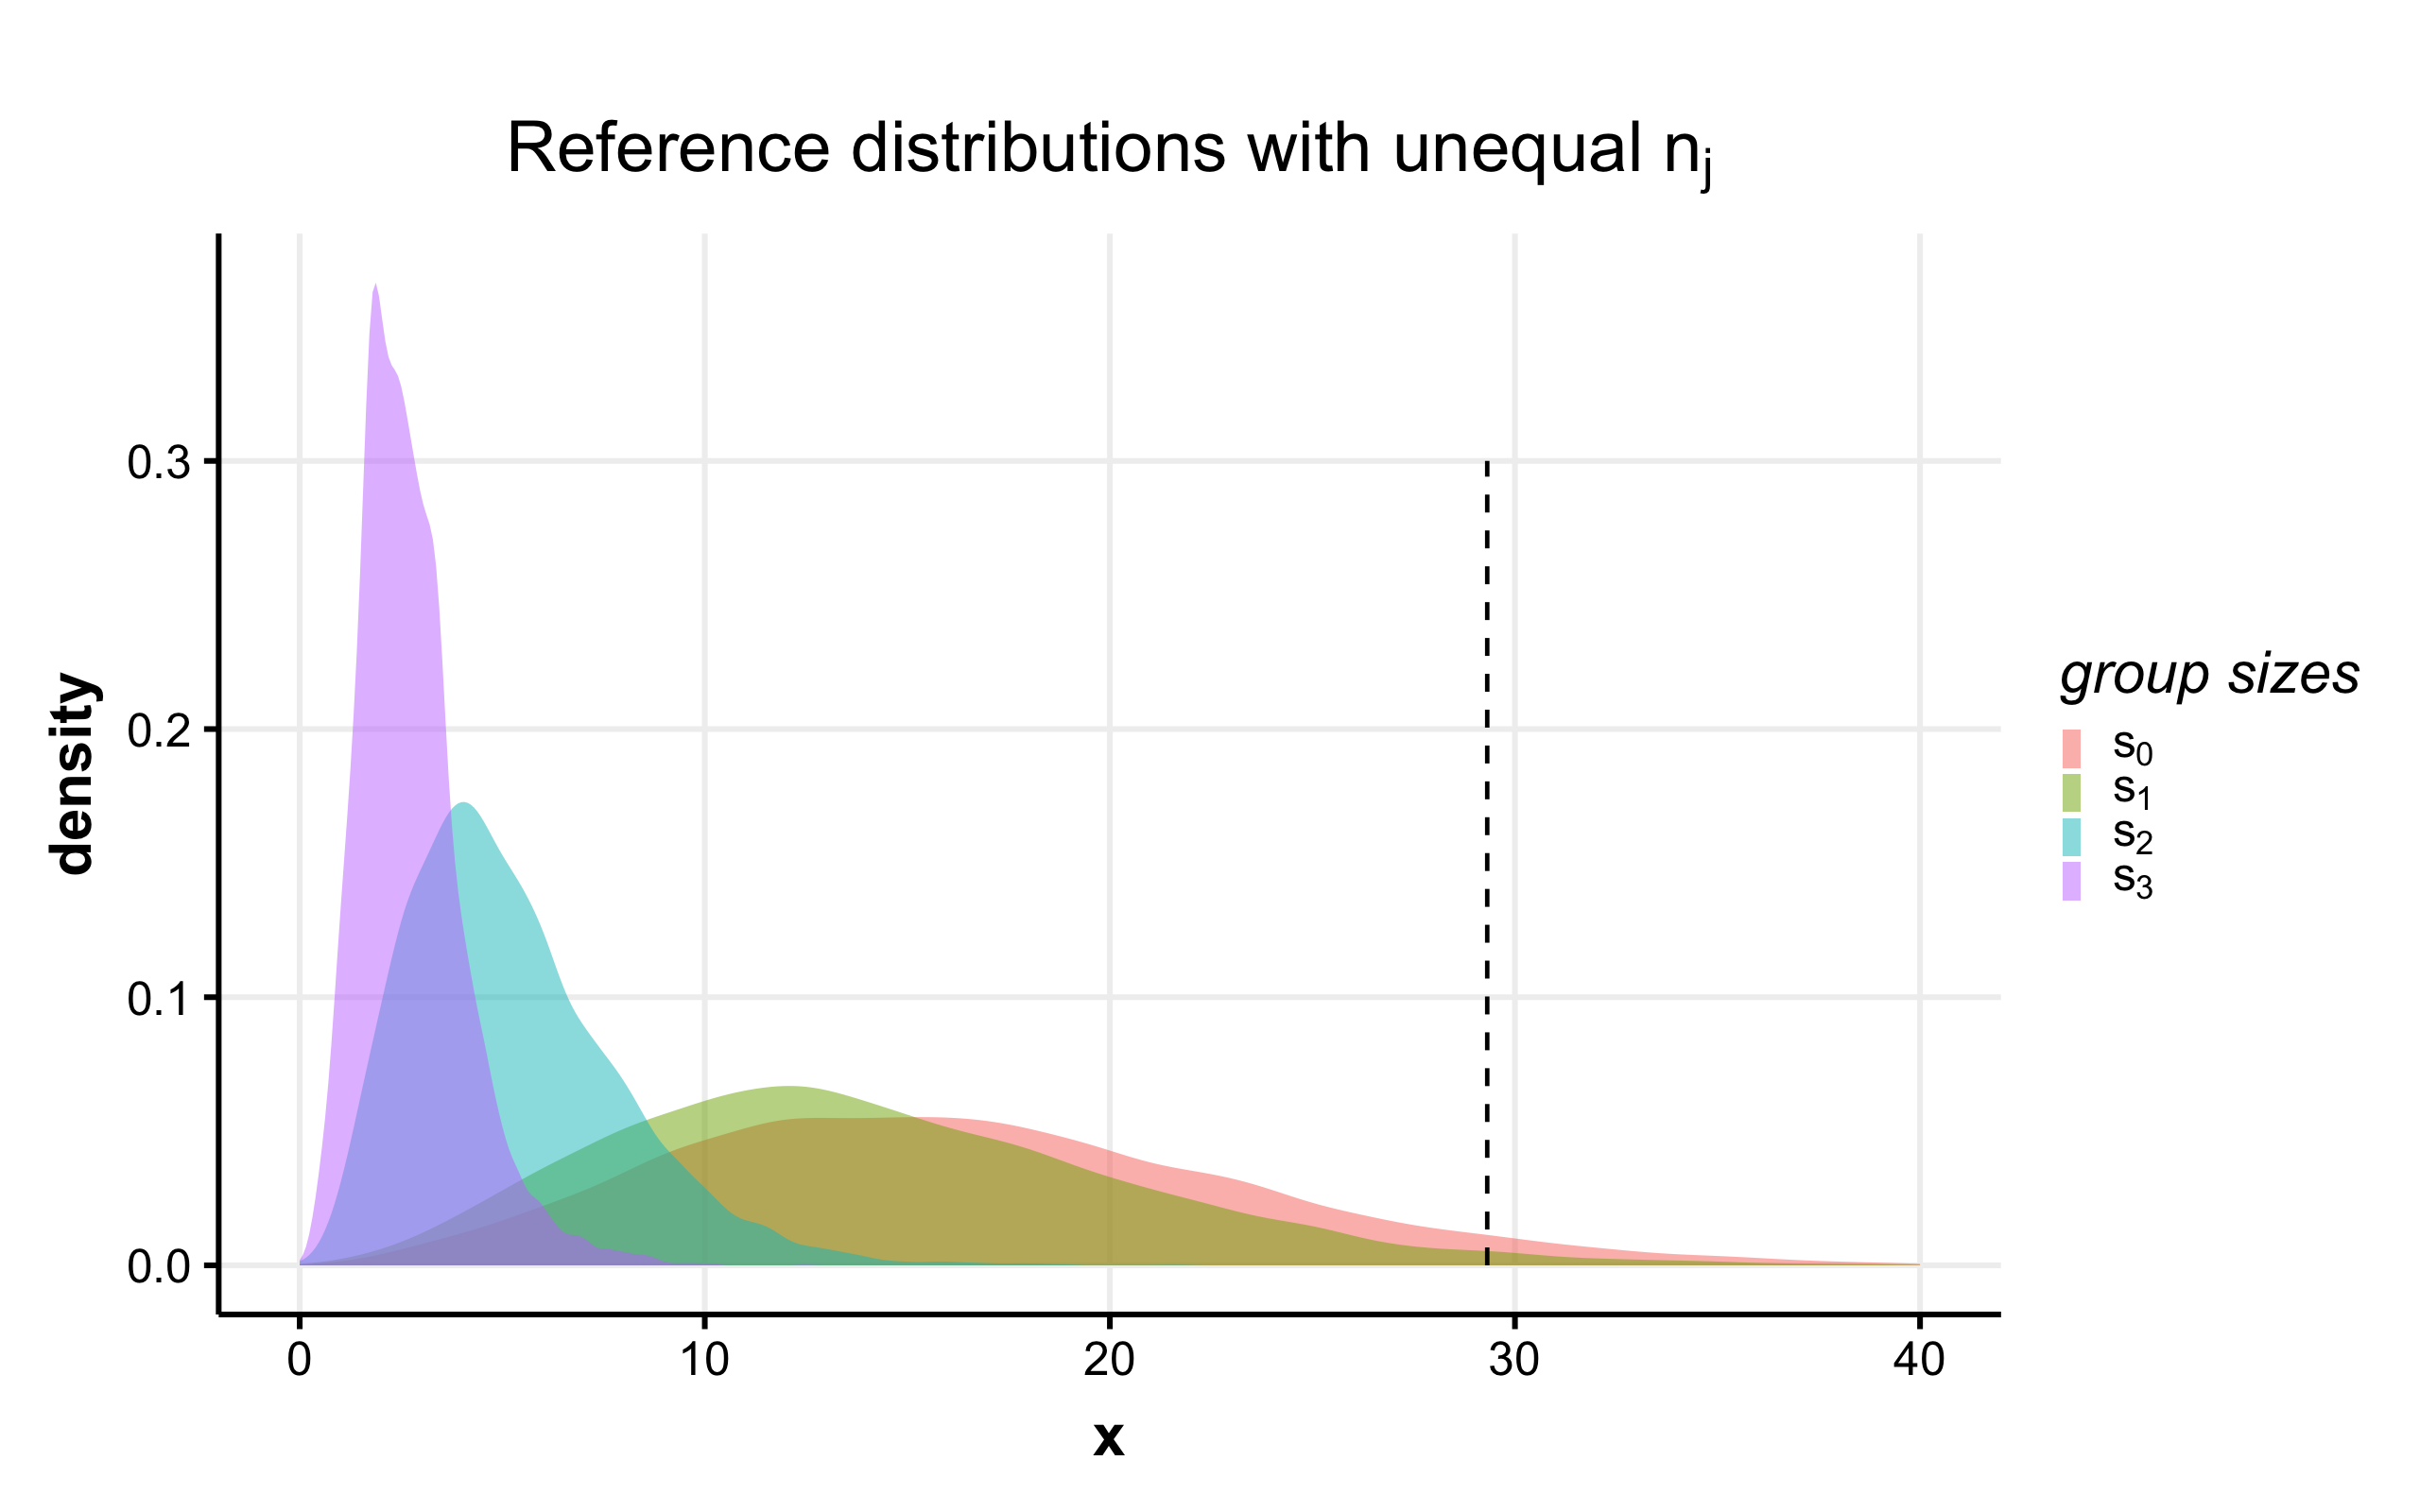
\includegraphics[width=\linewidth]{unequal-group-sizes.png}
\caption{Distribution of $\hat{F}_1$ under $H_0$ in four group size allocation scenarios, each with 10,000 simulations. $s_0\colon \{200, 200, 200, 200 \}$, $s_1\colon \{100, 100, 100, 500 \}$, $s_2\colon \{5, 10, 20, 765 \}$, $s_3\colon \{3, 3, 3, 791 \}$. The vertical dotted line indicates the .95 quantile of the equal group size distribution.\label{Fig:unequal-group-sizes}}
\end{figure}

In the following, we show that under any scenario, the expected value of the $F_1$ statistic is maximized when the group sizes are equal. Recall that the form of the statistic is
$$
F_1(\x) = \frac{\sa(\x)/(k-1)}{\se(\x)/(\dbsize-k)}.
$$

where
\begin{equation*}
\sa(\x) = \sum_{j=1}^k n_j |\yj - \yb|
\end{equation*}

and
\begin{equation*}
\se(\x) &= \sum_{i=1}^N \lvert y_{i} - \bar{y}_{c_i} \rvert.
\end{equation*}

Only $SA$ is a function of the $n_j$, so we restrict our attention to that term as $E(F_1)$ for different allocations will scale with $E(SA)$ by a multiplicative constant.

Denote each term in the summation $SA_j$. By using the approach used in Appendix~\ref{Sec:AppSig} to find the distribution of $y_i - y_{c_i}$, it can be shown that $\yj - \yb$ is distributed normal mean zero, and variance $\omega_j^2 = \frac{\sigma^2}{n_j} - \frac{\sigma^2}{N}$.
\begin{align*}
    \E(SA) &= \E\left(\sum_{j=1}^k SA_j\right) \\
    &= \sum_{j=1}^k \E(SA_j) \\
    &= \sum_{j=1}^k\E\left(n_j|\yj - \yb|\right) \\
    &= \sum_{j=1}^k\E\left(n_j|\frac{\omega_j(\yj - \yb)}{\omega_j}|\right) \\
    &= \sum_{j=1}^kn_j\omega_j\E\left(|\frac{(\yj - \yb)}{\omega_j}|\right) &&\text{since } \omega_j > 0 \\
    &= \sum_{j=1}^kn_j\omega_j(\sqrt{\frac{2}{\pi}})
\end{align*}

Since each $|\frac{(\yj - \yb)}{\omega_j}|$ is distributed standard half normal, the expectation of each evaluates to the constant $\sqrt{\frac{2}{\pi}}$. Now we may also factor out $\sigma$ from $\omega_j$, providing the final answer:
\begin{equation*}
    \E(SA) = \sigma(\sqrt{\frac{2}{\pi}})\sum_{j=1}^kn_j\sqrt{\frac{1}{n_j} - \frac{1}{N}}.
\end{equation*}

\begin{prop}
The expectation of $SA$ is maximized when group sizes are all equal, i.e., when $n_j = n_{j'}$, for all $j \neq j'$
\end{prop}

\begin{proof}
It suffices to show that the sum between any two summands of the expectation is maximized when the other $k-2$ group sizes are fixed, so we begin by fixing each $n_j$ except for $n_1$ and $n_2$, without loss of generality. Define $c = n_1 + n_2$ to be the sum between the two unfixed group sizes, so then the sum between the first two summands becomes:
\begin{align*}
&\sigma(\sqrt{\frac{2}{\pi}})(n_1\sqrt{\frac{1}{n_1} - \frac{1}{N}} + (c-n_1)\sqrt{\frac{1}{(c-n_1)} - \frac{1}{N}}) \\
&=\sigma(\sqrt{\frac{2}{\pi}})(\sqrt{n_1 - \frac{n_1^2}{N}} + \sqrt{(c-n_1) - \frac{(c-n_1)^2}{N}})
\end{align*}
since $n_1$ and $c-n_1 > 0$. Now factoring constants and differentiating with respect to $n_1$:
\begin{align*}
\frac{1}{\sigma(\sqrt{\frac{2}{\pi}})}\frac{d}{dn_1}\E(SA_1 \!+\! SA_2) =~~~~~~&\\
 \frac{\frac{2 (c-n_1)}{N}-1}{2 \sqrt{-\frac{(c-n_1)^2}{N}+c-n_1}}&+\frac{1-\frac{2 n_1}{N}}{2 \sqrt{n_1-\frac{n_1^2}{N}}},
\end{align*}
which has only one solution in $n_1$, when $n_1 = \frac{c}{2} =  \frac{n_1 + n_2}{2}$, which implies $n_1 = n_2$. This critical point is associated with a maximum expectation on the first two summands, as desired. Applying this result across all $n_j, n_{j'}$ pairs such that $j \neq j'$, will result in maximizing each summand of the expectation when all $n_j = n_{j'}$, hence maximizing $\E(SA)$.
\end{proof}